\section{作成したシステムの概要}
%---------------------------------------------
\subsection{LEDを用いた光通信}
\subsubsection{システムの概要}
光通信の構成図と動作の流れを図\ref{fig:compo_l}に示す．
Arduino IDE のシリアルモニタに文字を入力し，7 bit asciiコードから4進数にエンコードする．
同期LEDの光を照度センサ（フォトトランジスタ）で検知すると通信を開始する．
このLEDは通信中常に光っている．
変換した数字を4つのLEDに割り当て，LEDを光らせることで0，1，2，3からなる数列を表現する．
通信の開始と終了については，同期専用のLEDを用いて，これが光っている間通信するものとする．
受信側のArduinoに接続した照度センサを各LEDの正面に配置し，各照度センサが光を受け取ったら対応する数字を配列に格納する．
同期LEDの光を受け取らなくなったら通信を終了する．


\begin{figure}[bt]
    \centering
    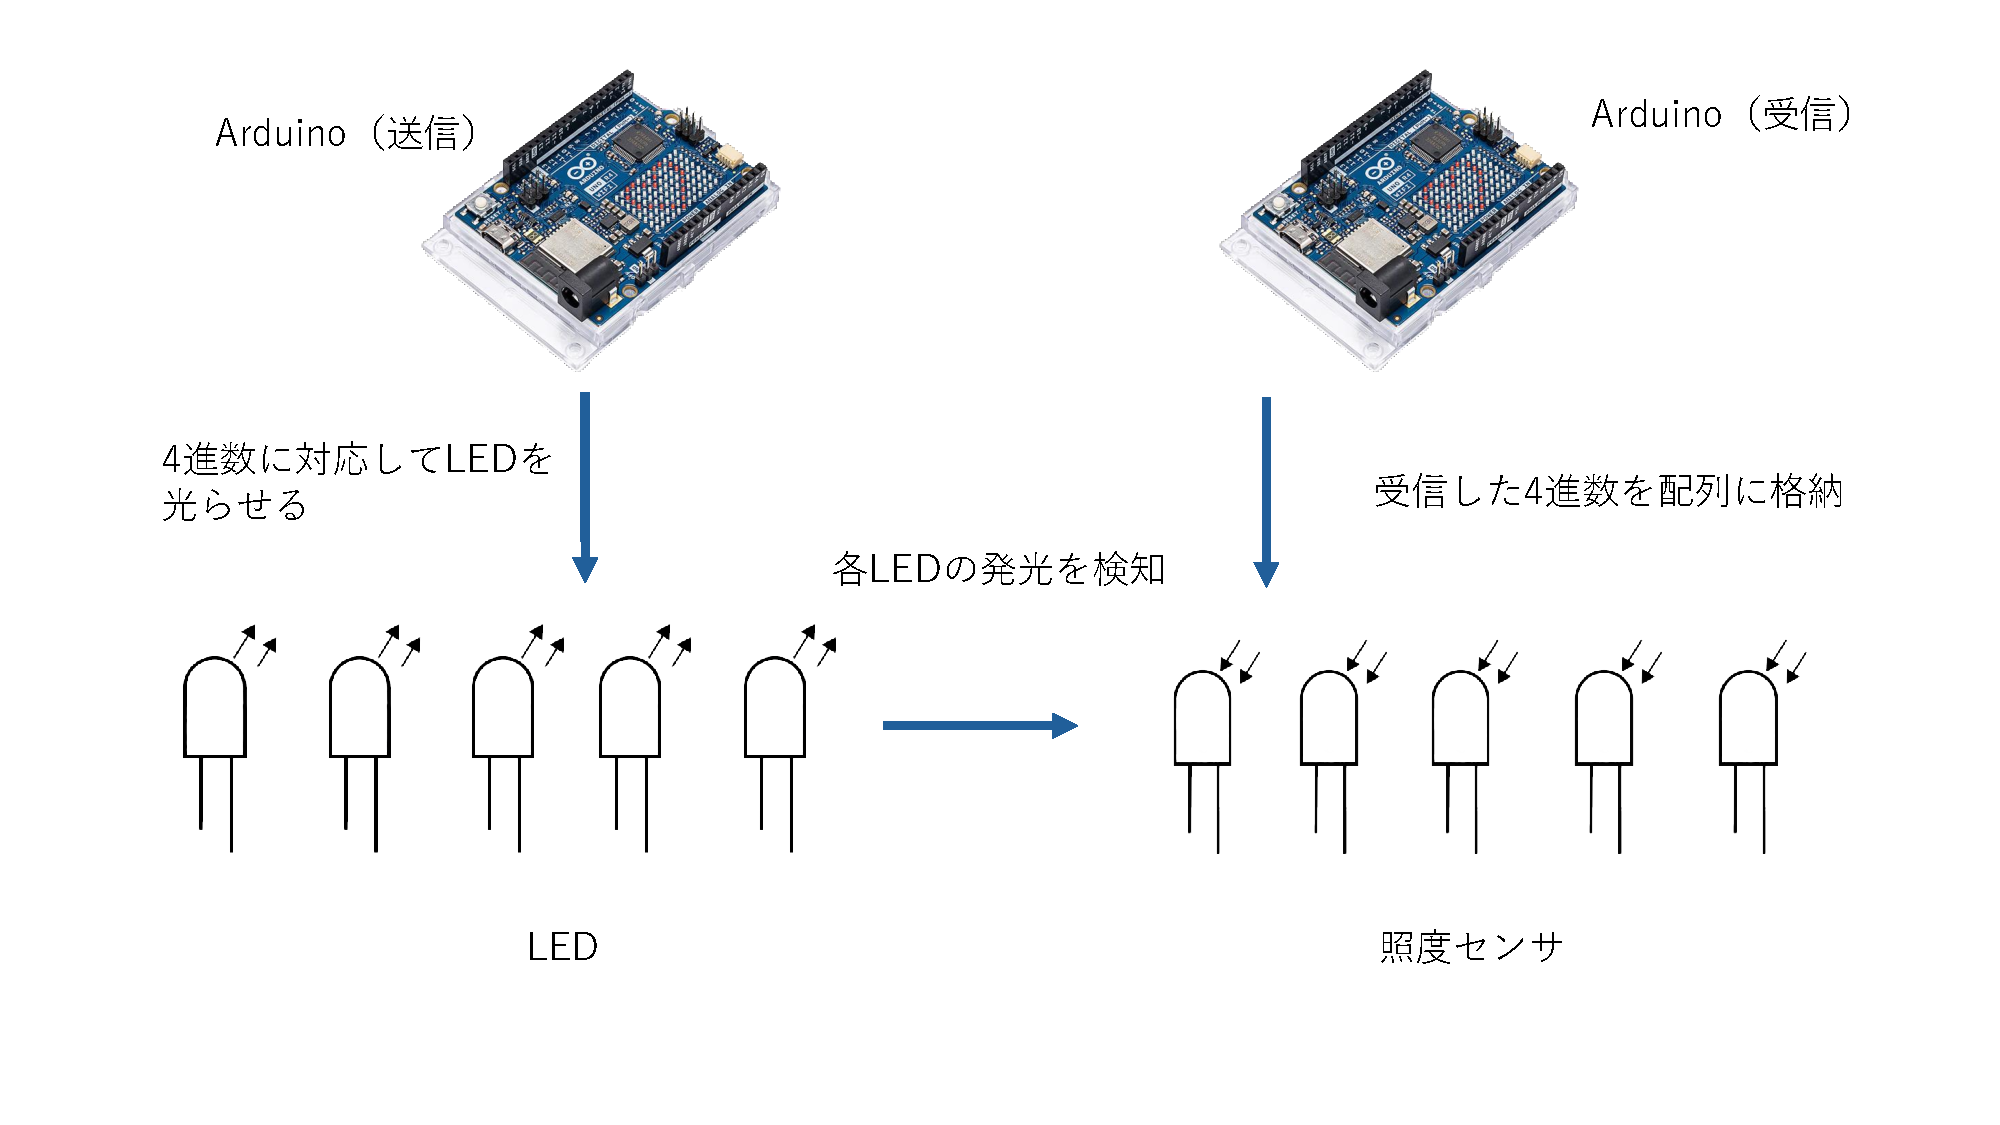
\includegraphics[width=\textwidth]{../img/compo_l}
    \caption{光通信の構成図と動作}
    \label{fig:compo_l}
\end{figure}



%-------------------------------------------------
\subsection{可聴音を用いた音通信}
\subsubsection{システムの概要}
音通信の構成図と動作の流れを図\ref{fig:compo_s}に示す．
通信開始は，同期専用の周波数を出力することで判断する．
光を受信して受け取った4進数の数列を2桁1シンボルに区切り，各シンボルに対応させた周波数の音をスピーカーから出力する．
それぞれの周波数をマイクで受け取ると，対応した文字列を4進数の数列に変換する．
同期周波数をもう一度検出すると通信を終了する．


\begin{figure}[bt]
    \centering
    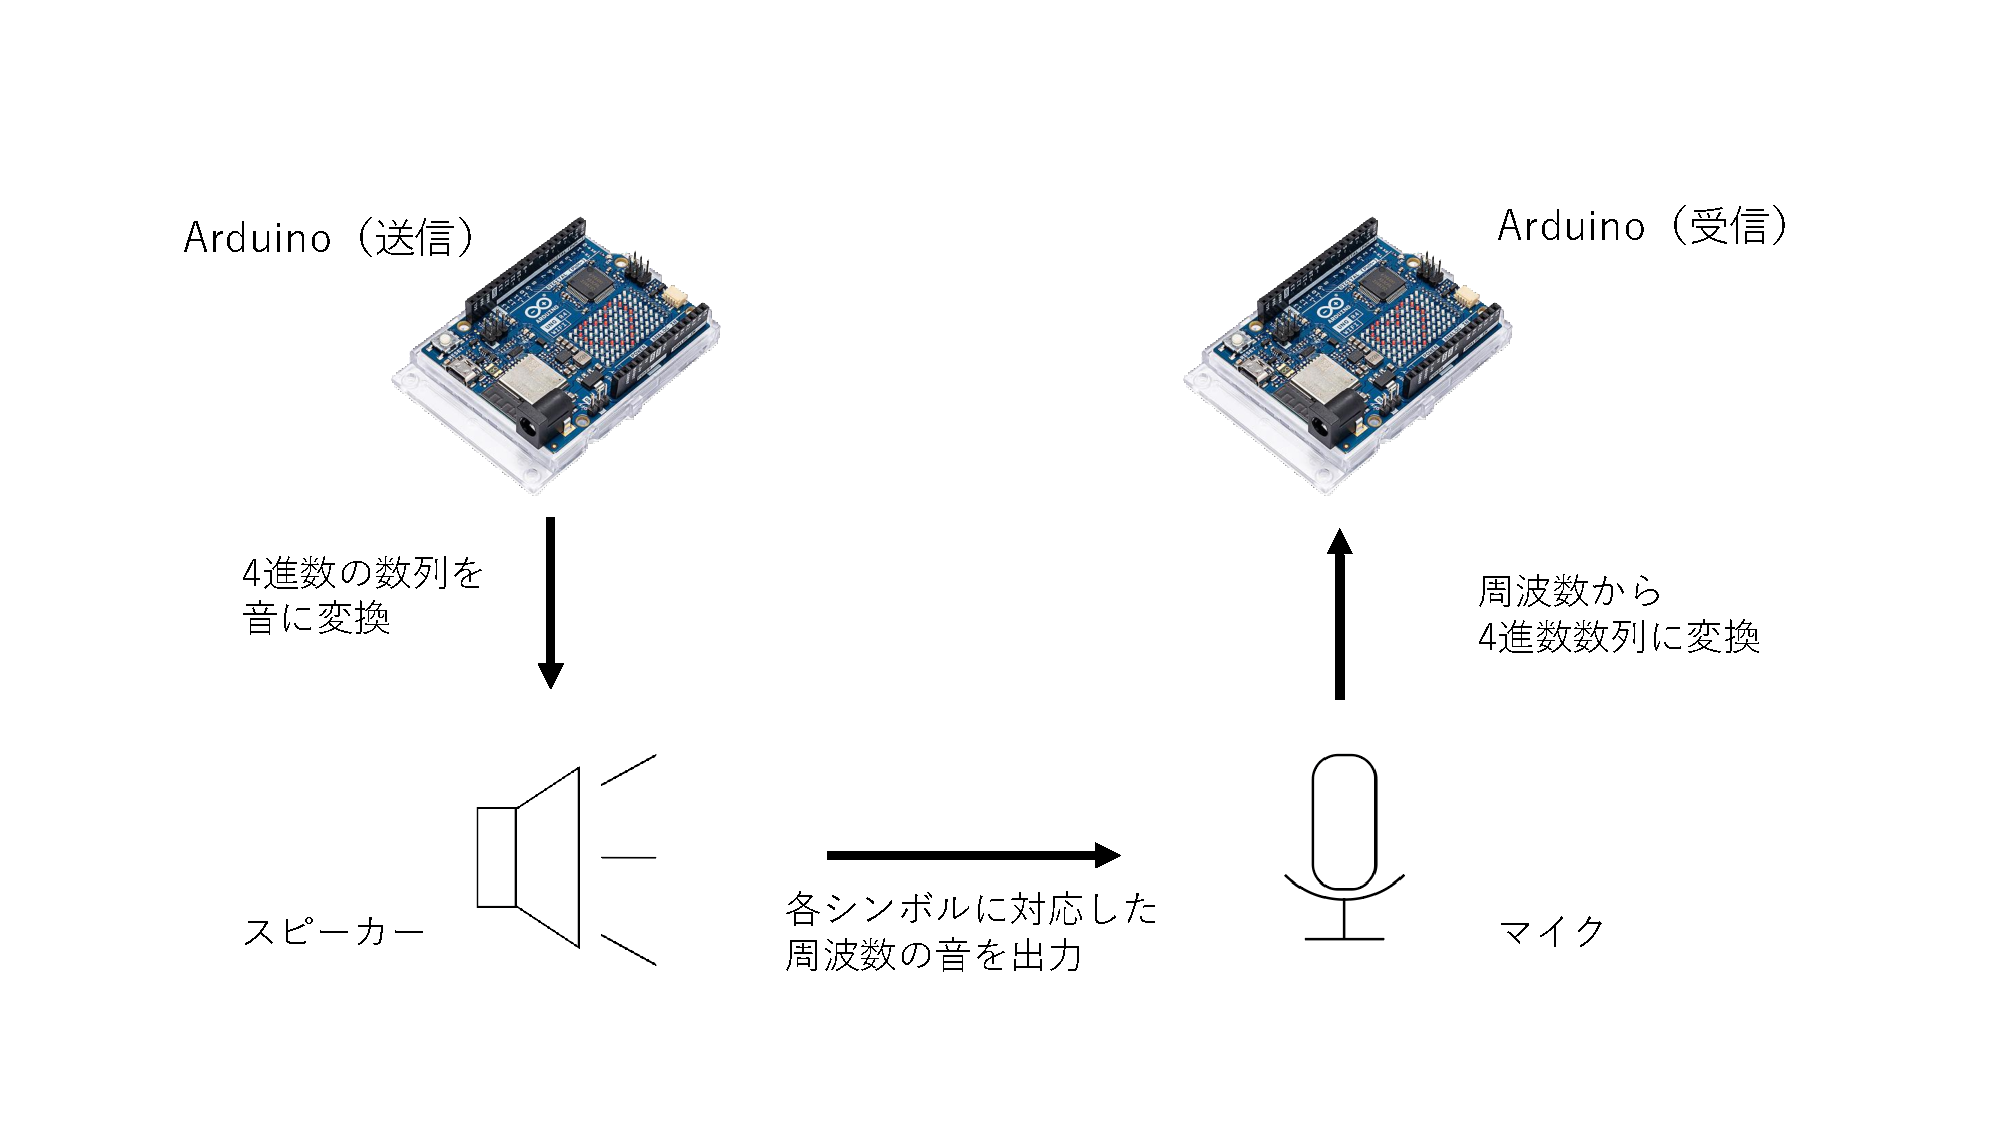
\includegraphics[width=\textwidth]{../img/compo_s}
    \caption{音通信の構成図と動作}
    \label{fig:compo_s}
\end{figure}


\subsubsection{出力する周波数とその検出}
送信側において，受け取った4進数の2桁と周波数と同期周波数の対応を表\ref{table:freq}に示す．
構想段階では同期周波数は1950 Hzだったが，環境音によって意図せず通信を開始，終了することがあったため，環境の影響を受けにくい3.6 kHzに変更した．
音と音の間に無音の時間（ガードインターバル：GI）を設ける．
これは隣り合うシンボルの干渉（シンボル間干渉：ISI）を軽減，防止するもので，GIをシンボル長の25 \%にすることで最低限の時間でISIを防ぎ，効率のよい通信が可能となる\cite{ref:gi}．
実際には，出力する音の長さを300 ms，GIを音長の25 \%に設定した．
受信側において，周波数の検出はarduinoFFTライブラリ（\url{https://github.com/kosme/arduinoFFT}）を用いて行った．
\begin{table}[bt]
    \centering
    \caption{受け取るシンボルと周波数の対応}
    \label{}
    \begin{tabular}{ccc} \hline
        シンボル（2桁） &周波数[kHz] \\ \hline
        同期周波数 &3.6 \\ \hline
        00 & 2.0\\ \hline
        01 & 2.1\\ \hline
        02 & 2.2\\ \hline
        03 & 2.3\\ \hline
        10 & 2.4\\ \hline
        11 & 2.5\\ \hline
        12 & 2.6\\ \hline
        13 & 2.7\\ \hline
        20 & 2.8\\ \hline
        21 & 2.9\\ \hline
        22 & 3.0\\ \hline
        23 & 3.1\\ \hline
        30 & 3.2\\ \hline
        31 & 3.3\\ \hline
        32 & 3.4\\ \hline
        33 & 3.5\\ \hline
    \end{tabular}
\end{table}

%----------------------------------------
\subsection{振動モータを用いた振動通信}
\subsubsection{システムの概要}
振動が7回連続したら通信を開始する．
音通信で受信した4進数の数列を7 bitのasciiコードに変換する．
変換したら各桁が0だったら振動をオフ，1だったら振動をオンにすることによって数列を送信する．
加速度センサによって3軸の加速度のベクトル距離を検知し，これが閾値を超えたら振動を検出する．
この振動の有無の検出により，振動を2進数に変換し，asciiコードを用いて具体的な文字にデコードする．
% -------------------------------------------------------------------------------------------
\subsection{システムの実装}
\subsubsection{使用した機器}
本システムに使用した機器を表\ref{table:devices}に示す．



\begin{table}[bt]
    \centering
    \caption{使用した機器}
    \label{table:devices}
    \begin{tabular}{|l|l|l|} \hline
        機器名                            &仕様          &個数  \\ \hline
        Arduino Uno R4 WiFi              &ABX00087     &3  \\ \hline
        ブレッドボード                      &EIC-102J      &3  \\ \hline
        発光ダイオード                      &              &5  \\ \hline
        フォトトランジスタ                  &NJL7502L       &5  \\ \hline
        ブレッドボード用ダイナミックスピーカ   &MSI28-12R      &1  \\ \hline
        マイクアンプモジュール               &AE-MICAMP      &1  \\ \hline
        振動モータ                         &316040001      &1  \\ \hline
        3軸加速度センサ                    &KXR94-2050      &1  \\ \hline
        ダイオード                        &                &1  \\ \hline
        トランジスタ                       &                &1  \\ \hline
        炭素被膜抵抗器                     &22 $\Omega$     &1 \\ \hline
        炭素皮膜抵抗器                     &330 $\Omega$    &5 \\ \hline
        炭素皮膜抵抗器                     &3.3 k$\Omega$   &1 \\ hline
        炭素皮膜抵抗器                     &100 k$\Omega$   &5 \\ \hline
    \end{tabular}
\end{table}



\subsubsection{回路図とフローチャート}
各通信の回路図を図\ref{fig:circuit_l}，図\ref{fig:circuit_ls}，図\ref{fig:circuit_sv}，図\ref{fig:circuit_v}に，フローチャートを図\ref{fig:flow_l}図\ref{fig:flow_ls}図\ref{fig:flow_sv}図\ref{fig:flow_v}に示す．


\begin{figure}[bt]
    \centering
    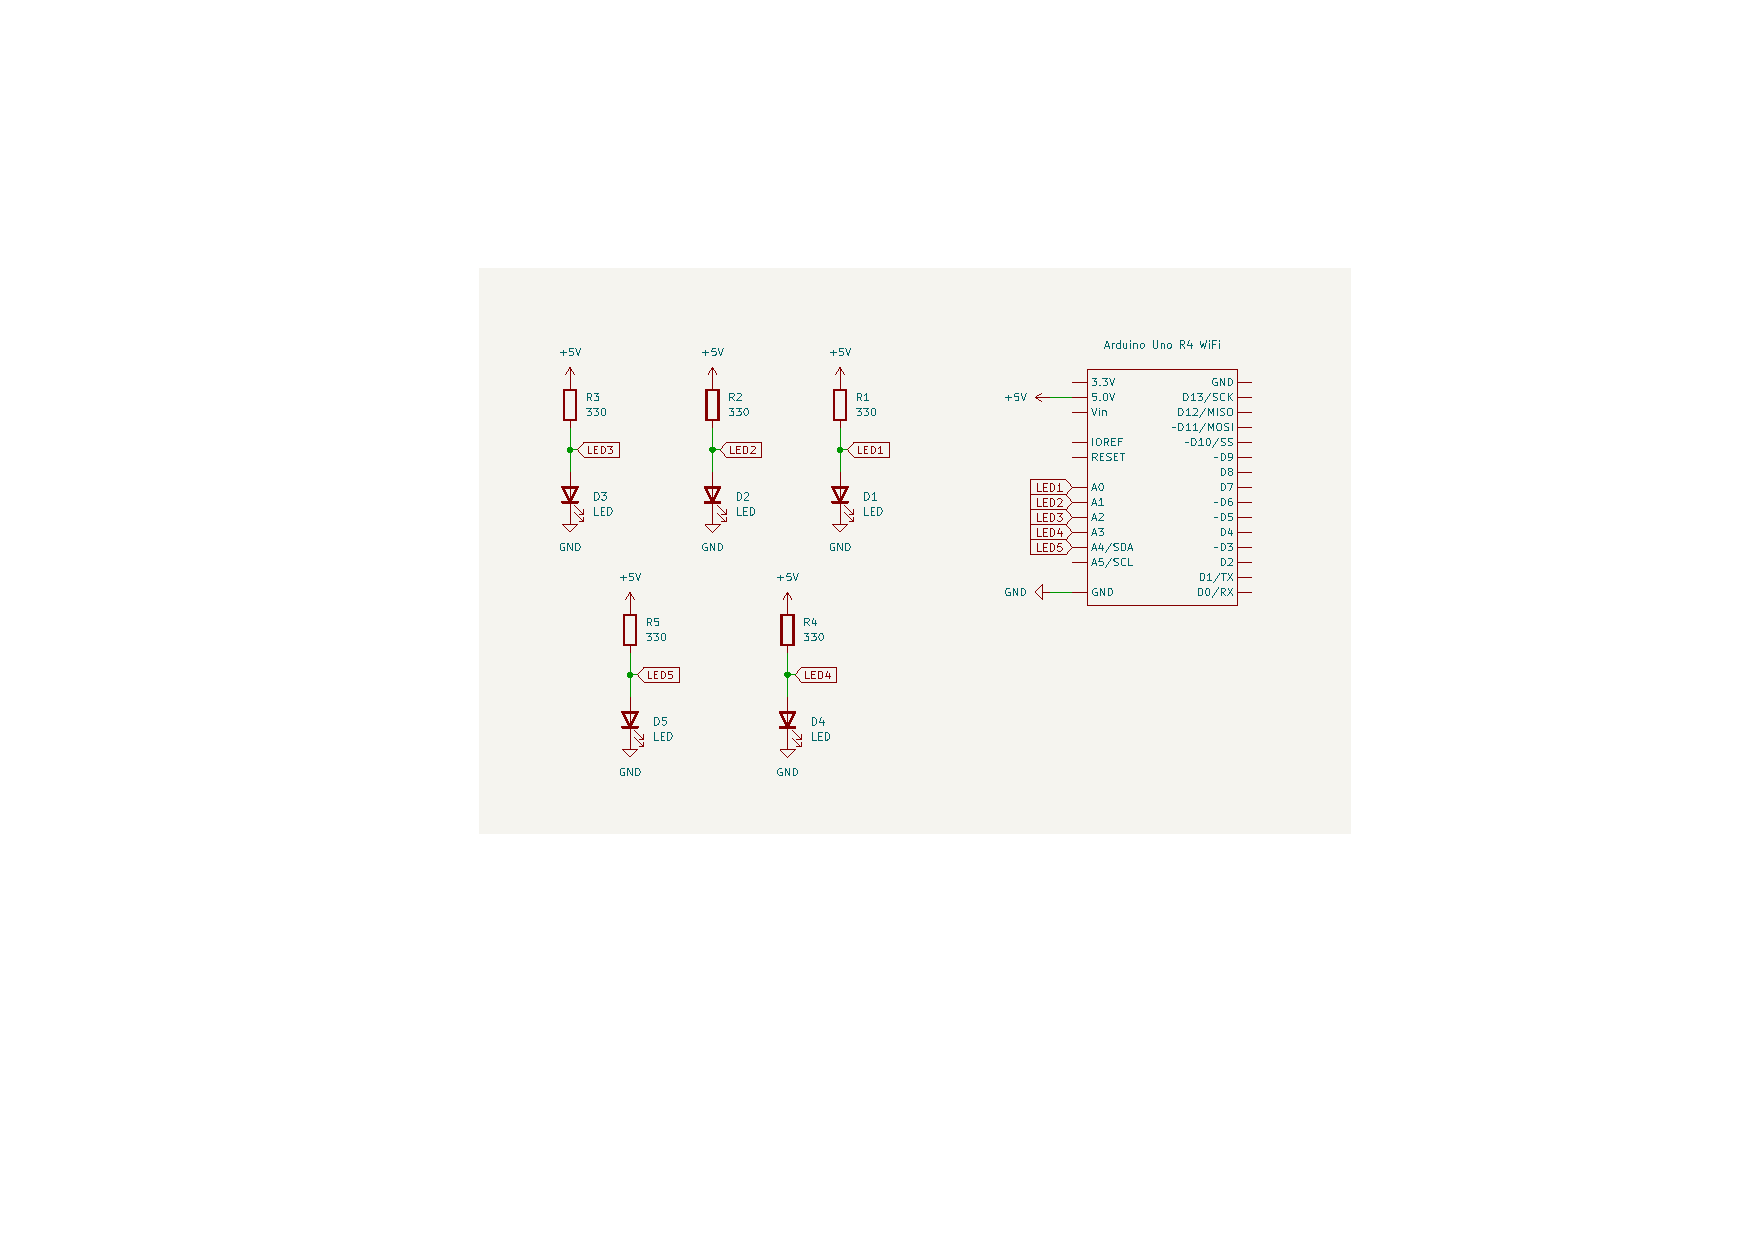
\includegraphics[width=120mm]{../img/circuit/ltx.pdf}
    \caption{光送信の回路図}
    \label{fig:circuit_l}
\end{figure}
\begin{figure}[bt]
    \centering
    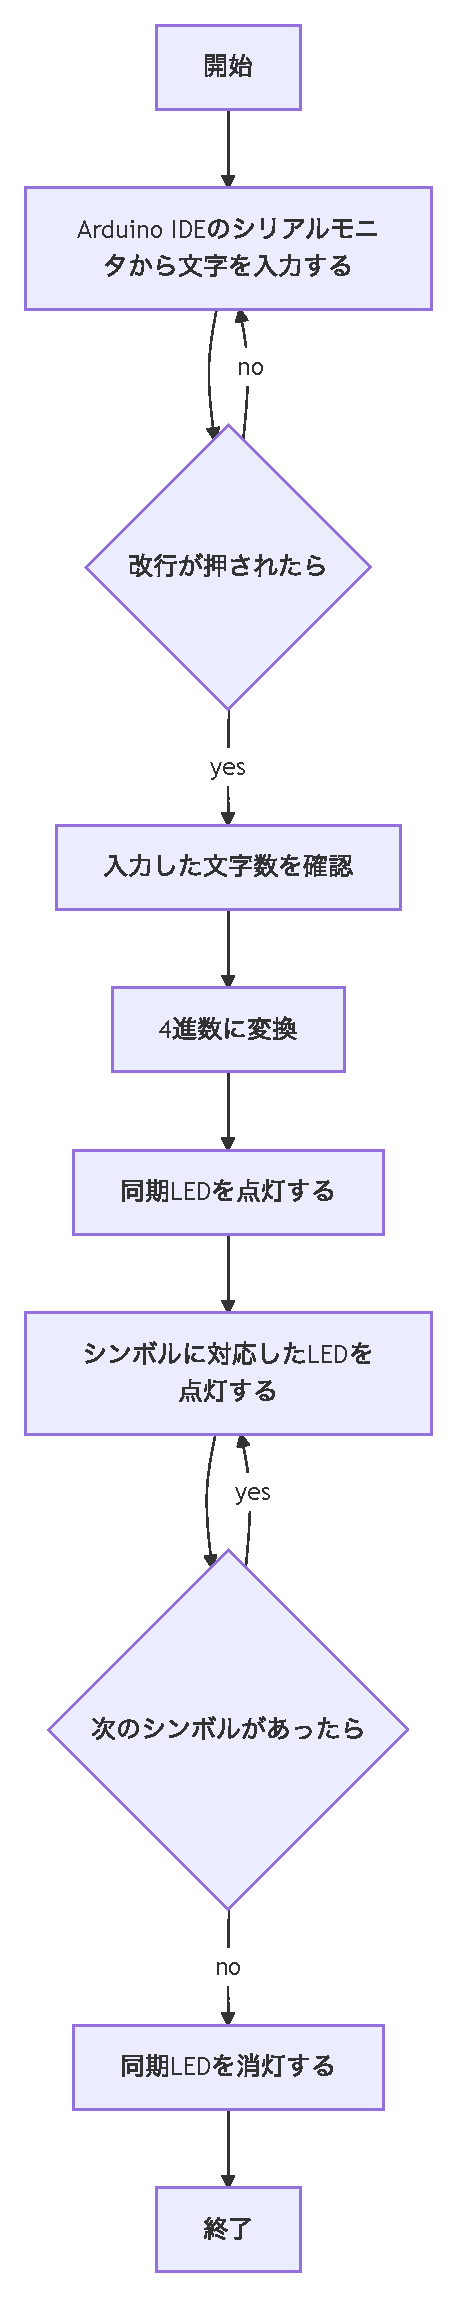
\includegraphics[height=\textheight]{../img/flow_ltx-1.pdf}
    \caption{光送信のフローチャート}
    \label{fig:flow_l}
\end{figure}

\begin{figure}[bt]
    \centering
    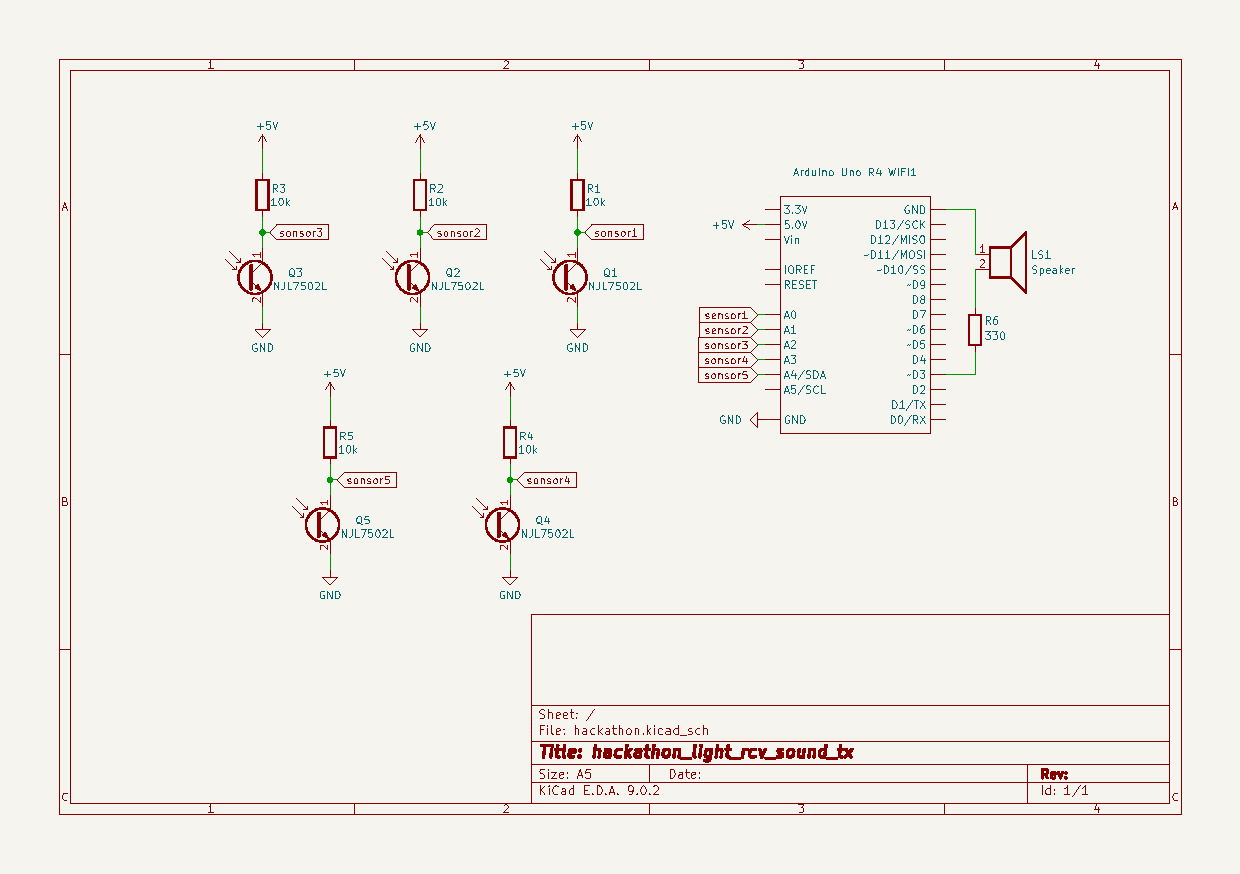
\includegraphics[width=120mm]{../img/circuit/lrcv_stx.pdf}
    \caption{光受信から音送信の回路図}
    \label{fig:circuit_ls}
\end{figure}
\begin{figure}[bt]
    \centering
    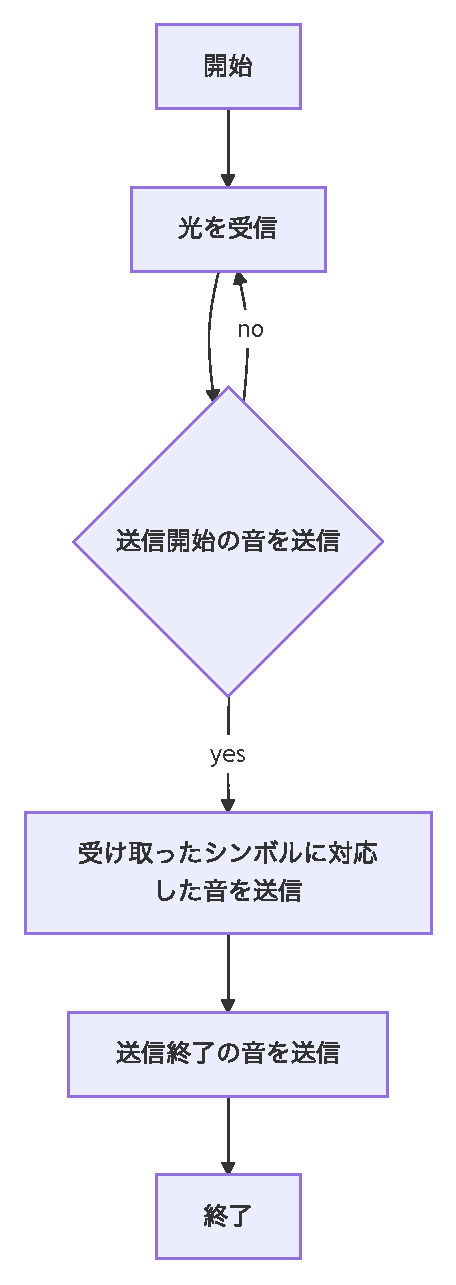
\includegraphics[width=\textheight]{../img/flow_stx-1.pdf}
    \caption{光受信から音送信のフローチャート}
    \label{fig:flow_ls}
\end{figure}

\begin{figure}[bt]
    \centering
    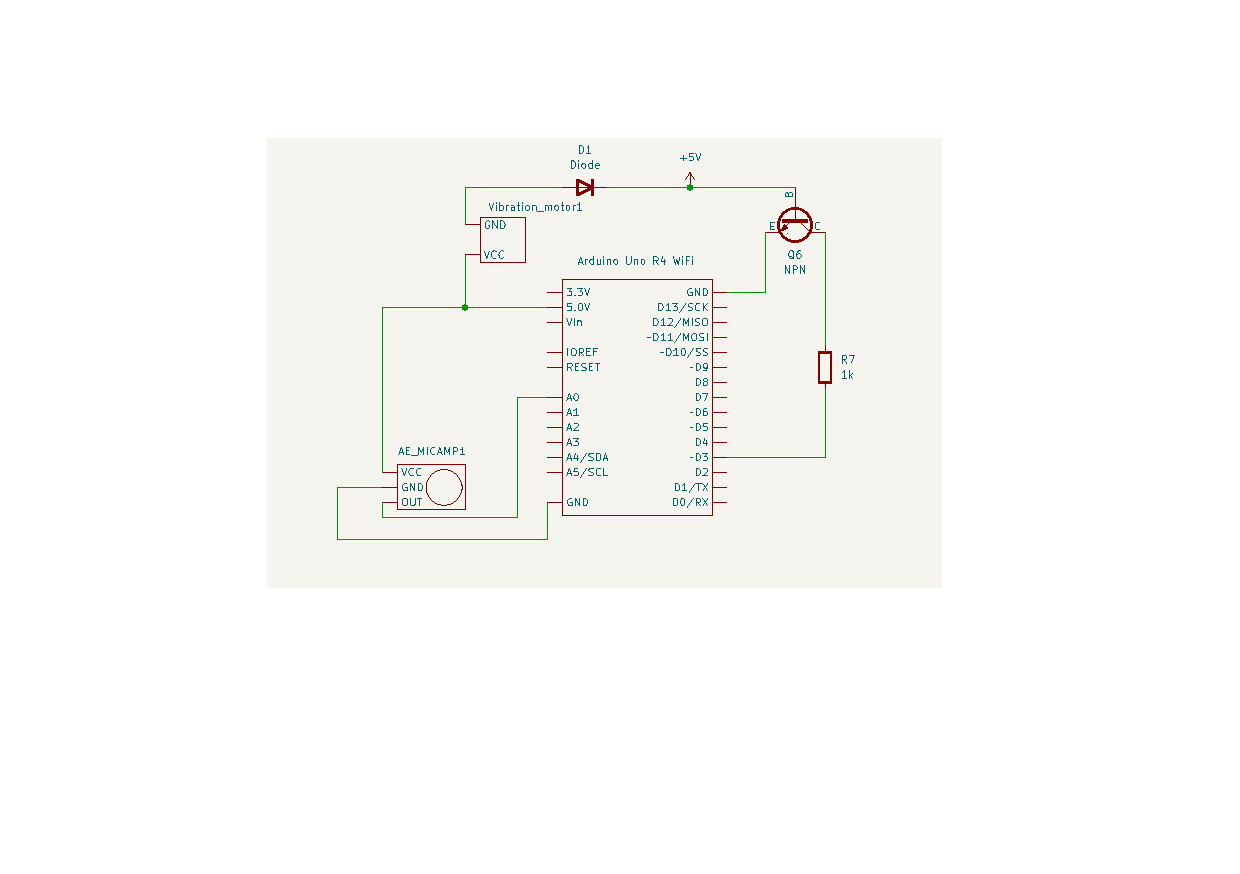
\includegraphics[width=120mm]{../img/circuit/srcv_vtx.pdf}
    \caption{音受信から振動送信の回路図}
    \label{fig:circuit_sv}
\end{figure}
\begin{figure}[bt]
    \centering
    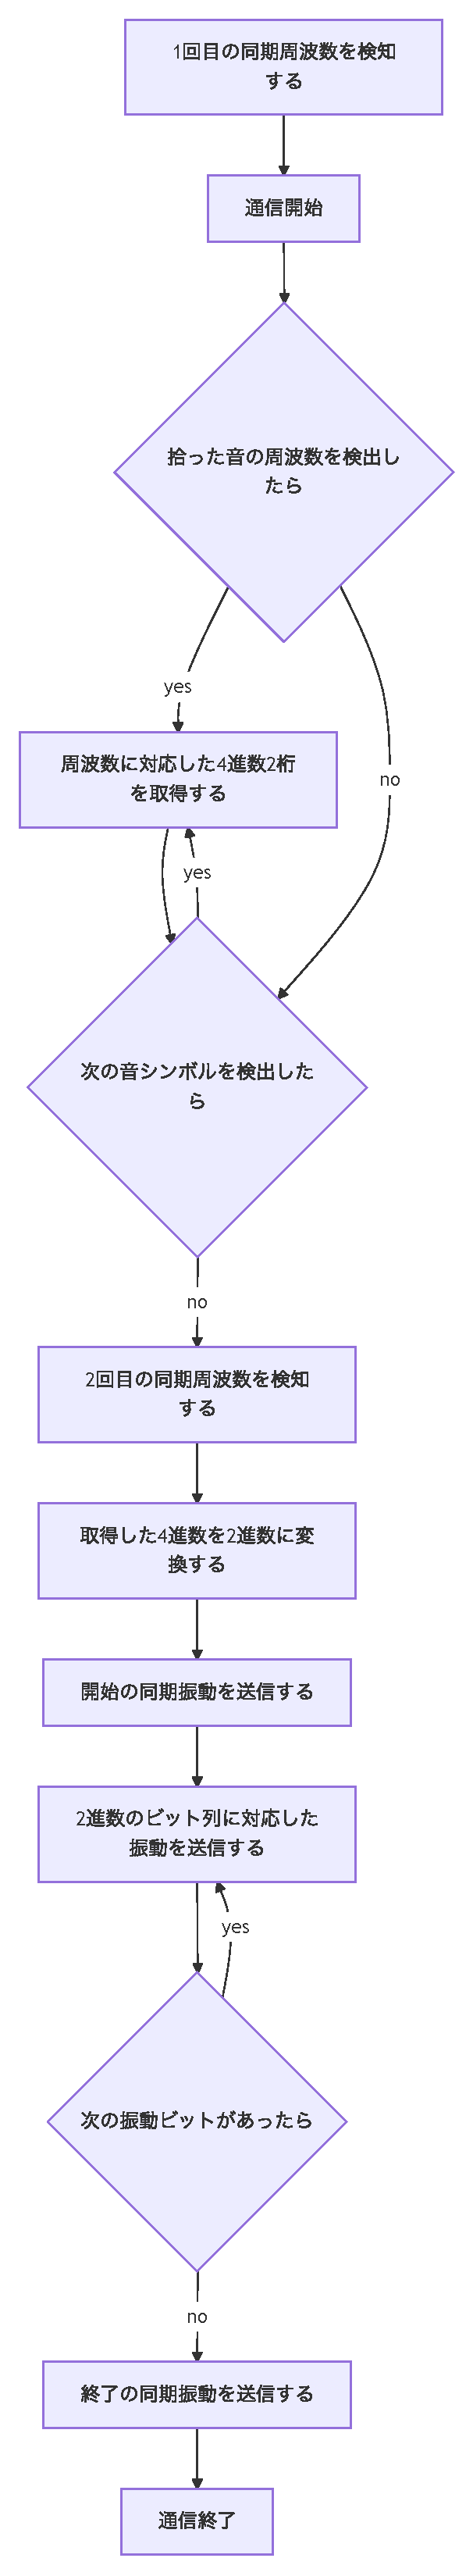
\includegraphics[width=\textheight]{../img/flow_vtx-1.pdf}
    \caption{音受信から振動送信のフローチャート}
    \label{fig:flow_sv}
\end{figure}

\begin{figure}[bt]
    \centering
    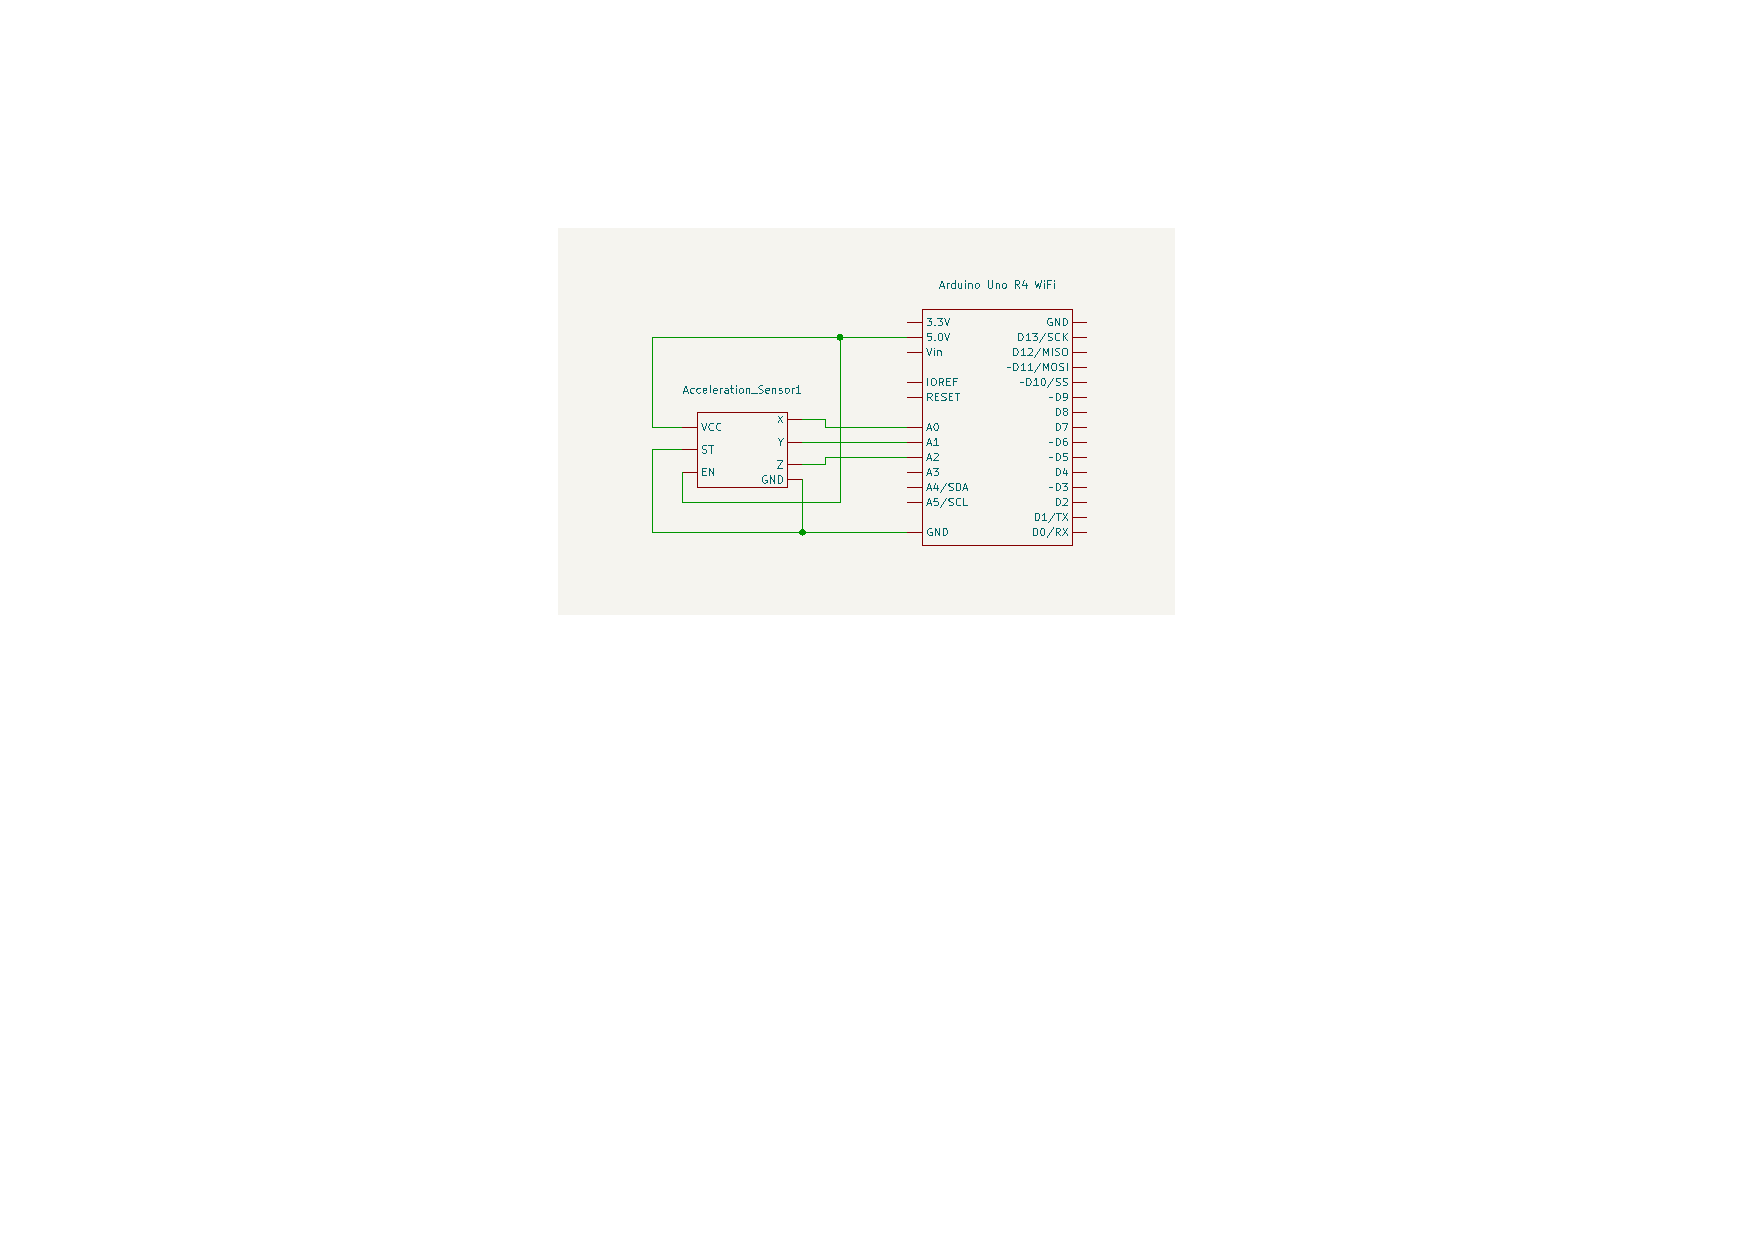
\includegraphics[width=120mm]{../img/circuit/vrcv.pdf}
    \caption{振動送信の回路図}
    \label{fig:circuit_v}
\end{figure}\begin{figure}[bt]
    \centering
    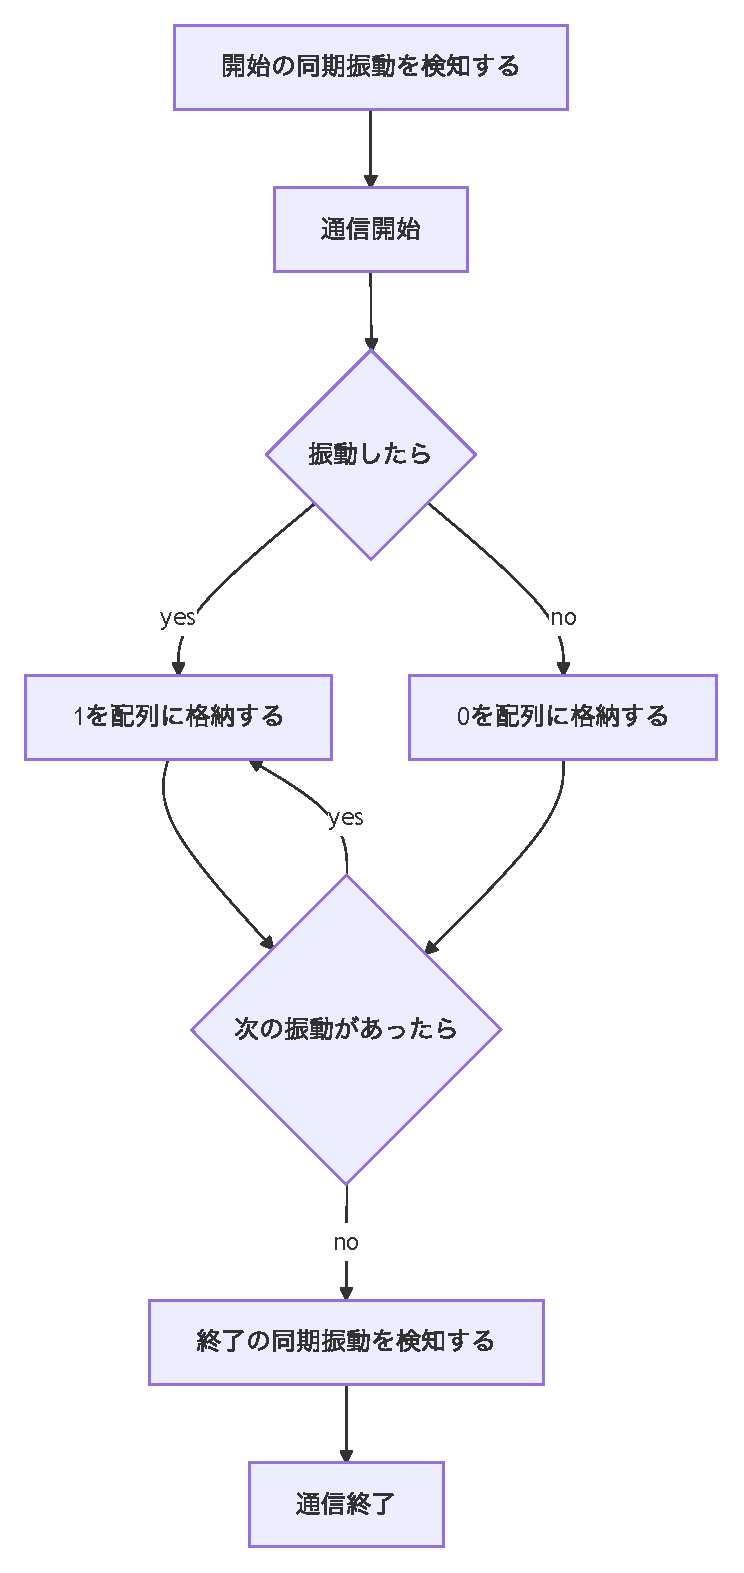
\includegraphics[width=\textheight]{../img/flow_vrcv-1.pdf}
    \caption{光送信のフローチャート}
    \label{fig:flow_v}
\end{figure}

\subsubsection{主要な関数の機能}
本システムにおけるArduinoスケッチの主要な関数の機能を説明する．

\begin{description}
    \item[detectBitByDuration関数（光受信）]
    閾値以上の光があると有効としてそのピンに対応するシンボルを保存する．
    \item[detectFrequency関数（音受信）]
    arduinoFFTライブラリを用いて，FFTでピーク周波数を検出する．
    \item[decodeFrequency関数（音受信）]
    開始，終了の同期周波数とシンボル周波数から4進数2桁のデータに変換する．
    \item[detectVibration関数（振動受信）]
    一定時間内に振動の有無を判断，2進数データに変換し保存する．
\end{description}

